\documentclass{summarysheet}

\begin{document}

\maketitle{7}{The Momentum Principle}


\begin{multicols}{2}

\begin{topicbox}{Momentum}

\noindent The \emph{momentum} of a particle is defined as
\begin{eqbox}
\vec{p} = m\vec{v}.
\end{eqbox}
Note that momentum has units of kg\,m/s and is a \emph{vector} -- it points in the same direction as the velocity $\vec{v}$.

We can write Newton's second law in terms of momentum:
\[
\vec{F} = m\vec{a} = m\frac{d\vec{v}}{dt} = \frac{d(m\vec{v})}{dt} = \frac{d\vec{p}}{dt}.
\]
In words, this says that a force on an object changes the object's momentum.
\end{topicbox}


\begin{topicbox}{The Momentum Principle}

\noindent Now we can put these two new concepts to use.  Starting from
\[
\vec{F} = \frac{d\vec{p}}{dt},
\]
multiple both sides by $dt$ and integrate from $t = t_i$ to $t = t_f$:
\[
\int_{t_i}^{t_f} \vec{F} \, dt = \int_{\vec{p}_i}^{\vec{p}_f} d\vec{p}.
\]
The left hand side is the impulse $\vec{J}$, and the right hand side is $\Delta \vec{p} = \vec{p}_f - \vec{p}_i$.  The \emph{momentum principle} is a restatement of Newton's second law that says
\begin{eqbox}
\Delta \vec{p} = \vec{J}.
\end{eqbox} 
An impulse delivered to an object changes its momentum.

\end{topicbox}

\begin{topicbox}{Conservation of Momentum}

\begin{multicols}{2}

\noindent For a system of $N$ particles, the \emph{total} momentum $\vec{P}$ (that's a capital P!) is the sum of the individual particle momenta:
\begin{eqbox}
\vec{P} = \vec{p}_1 + \vec{p}_2 + \vec{p}_3 + \dots = \sum_{k=1}^N \vec{p}_k.
\end{eqbox}

\begin{center}
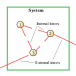
\includegraphics[scale=0.5]{fig_ext.pdf}
\end{center}


\end{multicols}
Thanks to Newton's third law, the sum of all the internal interaction forces is zero, so Newton's second law applies to the whole 
system,
\[
\vec{F}_\text{net} = \frac{d\vec{P}}{dt},
\]
where $\vec{F}_\text{net}$ is the sum of all \emph{external forces} only.

Now, if the net external force is \emph{zero}, $F_\text{net} = 0$, we call the system \emph{isolated}.  In that case, the total momentum of the system doesn't change -- it is \emph{conserved}:
\begin{eqbox}
\text{ \textsc{Law of Conservation of Momentum:}} \quad \vec{P}_i = \vec{P}_f.
\end{eqbox}
\end{topicbox}

\begin{topicbox}{Impulse}

\begin{multicols}{2}

\noindent The \emph{impulse} is defined as
\begin{eqbox}
\vec{J} = \int_{t_i}^{t_f} \vec{F} (t) \, dt.
\end{eqbox}

In a plot of the force (say, along the $x$-direction to makes things simpler) versus time, the impulse is the \emph{area under the force curve} from time $t = t_i$ to $t=t_f$.

\begin{center}
\includegraphics[scale=0.5]{fig_ft.pdf}
\end{center}


\end{multicols}

\end{topicbox}



\begin{topicbox}{APPLICATION: Collisions}

\noindent \textbf{Inelastic Collisions}

\noindent In an inelastic collision, two objects collide and stick together -- they have a common final velocity.  In an isolated system, momentum is conserved:
\begin{eqbox}
m_1 \vec{v}_{1i} + m_2 \vec{v}_{2i} = (m_1 + m_2) \vec{v}_f.
\end{eqbox}
\begin{center}
\includegraphics[scale=0.6]{fig_coll.pdf}
\end{center}

\noindent \textbf{Elastic Collisions}

\noindent In an elastic collision, two objects collide and bounce off each other \emph{elastically} -- meaning the total energy is conserved.  In the case where object 2 is at rest and the motion is along a straight line, the final speeds of each object are
\begin{eqbox}
v_{1f} = \frac{m_1 - m_2}{m_1 + m_2} v_{1i}; \quad v_{2f} = \frac{2m_1}{m_1 + m_2} v_{1i}.
\end{eqbox}
\begin{center}

\includegraphics[scale=0.6]{fig_coll2.pdf}
\end{center}

\end{topicbox}

\begin{topicbox}{APPLICATION: Explosions}

\noindent In an explosion, one object breaks into two or more pieces. In an isolated system, momentum is conserved:
\begin{eqbox}
 M_\text{tot} \vec{v}_i = m_1 \vec{v}_{1f} + m_2 \vec{v}_{2f} + \dots
\end{eqbox}
\begin{center}
\includegraphics[scale=0.6]{fig_ex.pdf}
\end{center}


\end{topicbox}


\end{multicols}



\makebanner{Mechanics}

\end{document}



